\documentclass[class=article, crop=false]{standalone}
%\usepackage[subpreambles=true]{standalone}
\usepackage{import}
%\usepackage{booktabs}
%\usepackage{tikz}

%\usepackage[utf8]{inputenc}
\usepackage[subpreambles=true]{standalone}
\usepackage{import}
\usepackage{pgfplots}
\pgfplotsset{compat=newest}
\usepgfplotslibrary{groupplots}
\usepgfplotslibrary{dateplot}
\usepackage{caption}
\usepackage{subcaption}
\usepackage{graphicx}
\usepackage{amsmath}
\usepackage{amssymb}
\usepackage[parfill]{parskip}
\usepackage{float}

% \usepackage{pgfplots}
% \usetikzlibrary{pgfplots.groupplots}
% \pgfplotsset{compat=1.9,height=0.3\textheight,legend cell align=left,tick scale binop=\times}
% \pgfplotsset{grid style={loosely dotted,color=darkgray!30!gray,line width=0.6pt},tick style={black,thin}}
% \pgfplotsset{every axis plot/.append style={line width=0.8pt}}
%
% \usepgfplotslibrary{external}
% % Für die Verwendung von 'external' müssen die folgenden Anpassungen in Abhängigkeit der
% % LaTeX Distribution durchgeführt werden:
%
% % fuer Texlive: pdflatex.exe -shell-escape -synctex=1 -interaction=nonstopmode %.tex
% \tikzexternalize[shell escape=-shell-escape]   % fuer TeXLive
%
% % fuer MikTeX:  pdflatex.exe -enable-write18 -synctex=1 -interaction=nonstopmode %.tex
% %\tikzexternalize[shell escape=-enable-write18] % fuer MikTex
%
%
%
% \tikzsetexternalprefix{graphics/pgfplots/} % Ordner muss ev. zuerst haendisch erstellt werden

\begin{document}

\subsection{Custom adaptive Kalman filter}\label{subsec:customkalman}
State estimation is an important part of any mobile robot. Its accuracy can be refined by multiple sensors. In order to deal with sensor noise and other inaccuracies during our position estimation, we used a linear quadratic estimator known as the Kalman Filter.

It is widely used in control theory and control systems engineering. Its applications include aircraft, spacecraft, ships and robot motion planning.

\subsubsection{Kalman Filter Theory}\label{subsubsec:kalmanfilter}

The Kalman Filter is a recursive digital filter that uses the system's dynamic model with uncertainties and noisy sensor measurements to estimate the system state while minimizing errors.

It uses a relative weight called the Kalman gain that is used with the current state estimation and sensor measurements. Its purpose is to "trust" values more that have a smaller uncertainty and thus give a more reliable estimation. It achieves that by the using covariances of the measurements and known, also to some extent unkown, noise that effect the states.

The following system model seen in \eqref{eq:generickalman} is a generic model of the Kalman Filter we used. It is based on a lecture script from Kemmetm{\"u}ller, W and Kugi, A\cite{regelungssysteme1} that is currently used in the Automation Master degree course Control Systems 1 at TU Vienna.

\begin{equation}
\begin{gathered}
  \textbf{x}_{k+1} =
  \boldsymbol{\Phi}_k
  \textbf{x}_k +
  \boldsymbol{\Gamma}_k
  \textbf{u}_k +
  \textbf{G}_k
  \textbf{w}_k \\
  \textbf{y}_k =
  \textbf{C}_k
  \textbf{x}_k +
  \textbf{D}_k
  \textbf{u}_k +
  \textbf{H}_k
  \textbf{w}_k +
  \textbf{v}_k \\
  \textbf{x}(0) = \textbf{x}_0 \\
\end{gathered}\label{eq:generickalman}
\end{equation}

The system consists of a state vector $ \textbf{x}_k  \in  \Re^n $, an input vector $ \textbf{u}_k \in \Re^p $, an output(measurement) vector $ \textbf{y}_k \in \Re^q $, a process noise vector $ \textbf{w}_k \in \Re^r $, a measurement noise vector $ \textbf{v}_k \in \Re^q $ and a time variant dynamic coefficient matrix $ \boldsymbol{\Phi}_k \in \Re^{n \times n}$,
an input coupling matrix $ \boldsymbol{\Gamma}_k \in \Re^{n \times p}$, a process noise input coupling matrix $ \boldsymbol{G}_k \in \Re^{n \times r} $, a measurement sensitivity matrix $ \boldsymbol{C}_k \in \Re^{q \times n} $, a measurement output coupling matrix $ \boldsymbol{D}_k \in \Re^{q \times p}$ and a process noise output coupling matrix $ \textbf{H}_k \in \Re^{q \times r} $.

\noindent
The following assumptions about the system were made:

\noindent
1. For the system noise vector $ \textbf{w}_k$ and measurement noise vector $ \textbf{v}_k $:
\begin{align*}
    E(\textbf{w}_k \textbf{w}_j^T) &= \textbf{R}_k \delta_{kj} & \textbf{R}_k &\ge \textbf{0} & E(\textbf{w}_k) &= \textbf{0} \\
    E(\textbf{v}_k \textbf{v}_j^T) &= \textbf{Q}_k \delta_{kj} & \textbf{Q}_k &\ge \textbf{0} & E(\textbf{v}_k) &= \textbf{0} \\
    E(\textbf{w}_k \textbf{v}_j^T) &= \textbf{0} & \textbf{H}_k  \textbf{Q}_k \textbf{H}_k^T &> \textbf{0}\\
\end{align*}\label{eq:assumption1}
Where $ \textbf{Q}_k \in \Re^{r \times r} $ is the process noise covariance matrix and $ \textbf{R}_k \in \Re^{q \times q} $ is the measurement noise covariance matrix and $ \delta_{kj} $ the Kroneckersymbol, which is $ \delta_{kj} = 1$ for $ k = j $ and $ \delta_{kj} = 0$ for $ k \neq j $.

\vspace{0.5cm}
\noindent
2. The expected value of the initial state vector $ \textbf{x}_0 $ and the initial state error covariance matrix $ \textbf{P}_0 $:
\begin{align*}
    E(\textbf{x}_0) &= \textbf{m}_0 & E([\textbf{x}_0 - \hat{\textbf{x}}_0][\textbf{x}_0 - \hat{\textbf{x}}_0]^T) &= \textbf{P}_0 \ge 0
\end{align*}\label{eq:assumption2}
Where $ \hat{\textbf{x}}_0 $ is a guess for the initial state vector $ \textbf{x}_0 $.

\noindent
3. The process noise vector $\textbf{w}_k$ and measurement noise vector $\textbf{v}_k$ are not correlated with the intial state vector $ \textbf{x}_0 $:
\begin{align*}
    E(\textbf{w}_k \textbf{x}_0^T) &= \textbf{0}\\
    E(\textbf{v}_k \textbf{x}_0^T)&= \textbf{0}\\
\end{align*}\label{eq:assumption3}
We modelled our system with the 5-dimensional state vector:

\begin{center}
 $\textbf{x}_k =
  \begin{bmatrix}
   x_k    \\
   y_k    \\
   v_k    \\
   \Psi_k \\
   \dot{\Psi}_k
  \end{bmatrix}
 $
\end{center}

where $x_k$ is the distance travelled in x, $y_k$ the distance travelled in y, $v_k$ is the robot's relative x speed, $\Psi_k$ is the yaw of the robot and $\dot{\Psi}_k$ is the yaw speed.

Our system input is a joystick controller, which we use to move our robot forward and backward by setting the motors to a certain speed or rotate it left or right by setting one of the motors forward and the other backward. We modelled this joystick input as:
\begin{center}
$ \textbf{u}_k =
\begin{bmatrix}
     \vartheta_k \\
     \eta_k    \\
 \end{bmatrix}
$
\end{center}

Where $\vartheta_k \in [-1,1]$ is our forwards and backwards signal and $\eta_k \in [-1,1]$ is our rotation signal in the right and left direction. The top speed of the motors, by setting $\vartheta_k = \pm 1$, is the constant $\alpha$ and the top turn speed at $\eta_k = \pm 1$ is the constant $\beta$.

Our system output $y_k$ is measured by our gyroscope and accelerometer in the IMU:
\begin{center}
 $ \textbf{y}_k =
  \begin{bmatrix}
   \zeta_k \\
   \chi_k  \\
  \end{bmatrix}
 $
\end{center}

where $\zeta_k$ is the acceleration measured in the x direction and $\chi_k$ is the measured yaw speed.

To construct our dynamic coefficient matrix $ \boldsymbol{\Phi_k} $ and input coupling matrix $ \boldsymbol{\Gamma_k} $, we used the following equations based on Newtonian motion dynamics and Euler method:
\begin{align*}
    x_{k+1} &= x_k + v_k \Delta t cos(\Psi_k)\\
    y_{k+1} &= y_k + v_k \Delta t sin(\Psi_k)\\
    v_{k+1} &= \alpha \vartheta_k\\
    \Psi_{k+1} &= \Psi_k + \Delta t \dot{\Psi}_{k}\\
    \dot{\Psi}_{k+1} &= \beta \eta_k \\
\end{align*}\label{eq:systemdyn}
For our measurement matrix and our measurement input matrix we used the following equations, also derived from Newtonian dynamics:
\begin{align*}
\zeta_k &= \frac{\alpha \vartheta - v_k}{\Delta t}\\
\chi_k &= \dot{\Psi}_{k}
\end{align*}\label{eq:outdyn}

The $\zeta_k$ estimation is a forwards difference, since $\alpha \vartheta$ gives us the robot speed in the next iteration, while $v_k$ is the current velocity.

Since we don't know the noise added to the system by our $\textbf{u}_k$ control input vector, we modelled it as an unknown system noise vector $\textbf{w}_k$ with a set standard deviation $\sigma$. The measurement noise vector $v_k$ was modelled similarly:
\begin{align*}
 \textbf{w}_k & = \begin{bmatrix}
  \sigma^{\vartheta_k}_k \\
  \sigma^{\eta_k}_k      \\
 \end{bmatrix} & \textbf{Q}_k & = \begin{bmatrix}
  (\sigma^{\vartheta_k}_k)^2 & 0                     \\
  0                          & (\sigma^{\eta_k}_k)^2 \\
 \end{bmatrix} \\
 \textbf{v}_k & = \begin{bmatrix}
  \sigma^{\zeta_k}_k \\
  \sigma^{\chi_k}_k  \\
 \end{bmatrix} & \textbf{R}_k & = \begin{bmatrix}
  (\sigma^{\zeta_k}_k)^2 & 0                     \\
  0                      & (\sigma^{\chi_k}_k)^2 \\
 \end{bmatrix} \\
\end{align*}\label{eq:noisemodel}
Putting together all of the previous equations into the form \eqref{eq:generickalman} we get:
\begin{align*}
    \begin{bmatrix}
     \hat{x}_{k+1}^-    \\
     \hat{y}_{k+1}^-    \\
     \hat{v}_{k+1}^-    \\
     \hat{\Psi}_{k+1}^- \\
     \hat{\dot{\Psi}}_{k+1}^- \\
    \end{bmatrix} &=
    \begin{bmatrix}
     1 & 0 & \Delta t sin(\hat{\Psi}_{k}^+) & 0 & 0 \\
     0 & 1 & \Delta t cos(\hat{\Psi}_{k}^+) & 0 & 0\\
     0 & 0 & 0                              & 0 & 0\\
     0 & 0 & 0                              & 1 & \Delta t\\
     0 & 0 & 0                              & 0 & 0
    \end{bmatrix}
    \begin{bmatrix}
     \hat{x}_{k}^+    \\
     \hat{y}_{k}^+    \\
     \hat{v}_{k}^+    \\
     \hat{\Psi}_{k}^+ \\
     \hat{\dot{\Psi}}_{k}^+
    \end{bmatrix} +
    \begin{bmatrix}
     0      & 0             \\
     0      & 0             \\
     \alpha & 0             \\
     0      & 0 \\
     0      & \beta \\
    \end{bmatrix}
    \begin{bmatrix}
     \vartheta_k \\
     \eta_k      \\
    \end{bmatrix} +
    \begin{bmatrix}
     0      & 0             \\
     0      & 0             \\
     \alpha & 0             \\
     0      & 0 \\
     0      & \beta \\
    \end{bmatrix}
    \begin{bmatrix}
     \sigma^{\vartheta_k}_k \\
     \sigma^{\eta_k}_k      \\
    \end{bmatrix}\\
    \begin{bmatrix}
     \zeta_k \\
     \chi_k  \\
    \end{bmatrix} &=
    \begin{bmatrix}
     0 & 0 & -\frac{1}{\Delta t} & 0 & 0 \\
     0 & 0 & 0                   & 0 & 1\\
    \end{bmatrix}
    \begin{bmatrix}
     \hat{x}_{k}^- \\
     \hat{y}_{k}^- \\
     \hat{v}_{k}^- \\
     \Psi_{k}^-    \\
     \dot{\Psi}_{k}^- \\
    \end{bmatrix} +
    \begin{bmatrix}
     \frac{\alpha}{\Delta t} & 0     \\
     0                       & 0 \\
    \end{bmatrix}
    \begin{bmatrix}
     \vartheta_k \\
     \eta_k      \\
    \end{bmatrix} +
    \begin{bmatrix}
     0 & 0 \\
     0 & 0 \\
    \end{bmatrix}
    \begin{bmatrix}
     \sigma^{\vartheta}_k \\
     \sigma^{\eta}_k      \\
    \end{bmatrix} +
    \begin{bmatrix}
     \sigma^{\zeta_k}_k \\
     \sigma^{\chi_k}_k  \\
    \end{bmatrix} \\
\end{align*}\label{eqn:fullsystem}
where the vector $\hat{\textbf{x}}_k^-$ is an "a priori" state estimation, the vector $\hat{\textbf{x}}_k^+$ is an "a posteriori" state estimation, which is an output corrected estimation of the "a priori" state, and an extrapolated $\hat{\textbf{x}}_{k+1}^+$, which then becomes the next iteration's "a priori" state.

The process noise input coupling matrix $\textbf{G}_k$ is filled with zeros(except for the input dimensions) because the process noise in the current iteration was already included by the last one in the $\hat{v}_{k}^-$, therefore it should not impact our current $\hat{x}_{k+1}^-$ and $\hat{y}_{k}^+$.

The process noise output coupling matrix $\textbf{H}_k$ was filled with zeros, because the process noise $\textbf{w}_k$ shouldn't impact our measurement $\textbf{y}_k$ since it is already included in $\hat{\textbf{x}}_{k}^-$.

Now that our system was constructed, we set the initial state vector $\textbf{x}_0 = \textbf{0}$ and the state error estimation matrix $\textbf{P}_0 = \textbf{0}$ and executed the following steps:

\noindent
1, Calculate Kalman gain matrix:
\vspace{0.5cm}
\begin{center}
$ \hat{\textbf{L}}_k = \textbf{P}^-_k \textbf{C}^T_k (\textbf{C}_k \textbf{P}^-_k \textbf{C}^T_k + \textbf{H}_k \textbf{Q}_k \textbf{H}^T_k + \textbf{R}_k)^{-1} $
\end{center}
\vspace{0.5cm}
2, Update state vector:
\vspace{0.5cm}
\begin{center}
$ \hat{\textbf{x}}^+_k = \hat{\textbf{x}}^-_k + \hat{\textbf{L}}_k (\textbf{y}_k - \textbf{C}_k \hat{\textbf{x}}^-_k - \textbf{D}_k \textbf{u}_k) $
\end{center}
\vspace{0.5cm}
3, Update state error covariance matrix:
\vspace{0.5cm}
\begin{center}
$ \textbf{P}^+_k = (\textbf{E} - \hat{\textbf{L}}_k \textbf{C}_k ) \textbf{P}^-_k $
\end{center}
\vspace{0.5cm}
4, Extrapolate state vector:
\vspace{0.5cm}
\begin{center}
$ \hat{\textbf{x}}^-_{k+1} = \boldsymbol{\Phi}_k \textbf{x}^+_k + \boldsymbol{\Gamma}_k \textbf{u}_k $
\end{center}
\vspace{0.5cm}
5, Extrapolate state error covariance matrix:
\vspace{0.5cm}
\begin{center}
$ \textbf{P}^-_{k+1} = \boldsymbol{\Phi}_k \textbf{P}^+_k \boldsymbol{\Phi}^T_k + \textbf{G}_k \textbf{Q}_k \textbf{G}^T_k $
\end{center}

\vspace{0.5cm}

Steps 2 and 3 are the "a posteriori" estimations, which were used in all of the figures in the thesis unless stated otherwise.

\subsubsection{Custom adaptive Kalman Filter}

Our model of the Kalman Filter doesn't accurately describe the real motion of our robot, since the joystick input signal has sudden jumps and due to robot inertia there is a delay before it reaches that top speed.

In order to combat this, we increase the process noise by increasing our noise covariance matrix during this delay.

We first intruduce a ratio matrix $\boldsymbol{\Upsilon}_k$ that describes our process noise covariance matrix $\textbf{Q}_k$ in relation to the measurement noise covariance matrix $\textbf{R}_k$:
\begin{align*}
 \textbf{Q}_k              & =  \boldsymbol{\Upsilon}_k \textbf{R}_k &
 \begin{bmatrix}
  (\sigma^{\vartheta_k}_k)^2 & 0                     \\
  0                          & (\sigma^{\eta_k}_k)^2 \\
 \end{bmatrix} & =  \begin{bmatrix}
  (\varrho_{\vartheta\zeta})^2 & 0      \\
  0      & (\varrho_{\eta\chi})^2 \\
 \end{bmatrix}
 \begin{bmatrix}
  (\sigma^{\zeta_k}_k)^2 & 0                     \\
  0                      & (\sigma^{\chi_k}_k)^2 \\
 \end{bmatrix}
\end{align*}\label{eq:ratio}

To respond to the jumps from our joystick we used a moving weighted window with a set length N.

We implmented a mirrored sigmoid curve using the logistic function in our moving weighted window due its ability to hold the peak relatively high before it decreases rapidly closer to its half-life.

We calculate the $w_k$ weights of a moving weighted window of length $N$ as:
\begin{align*}
 \textbf{x}_k & = \left\{ x:x = \dfrac{n}{N}, n \in (0,N) \right\}   \\
 \textbf{w}_k & = \dfrac{ 1 }{ 1 + e^{\alpha ( \textbf{x}_k - \frac{1}{2})} }
\end{align*}

\vspace{0.5cm}

\begin{figure}[H]
 \begin{center}
  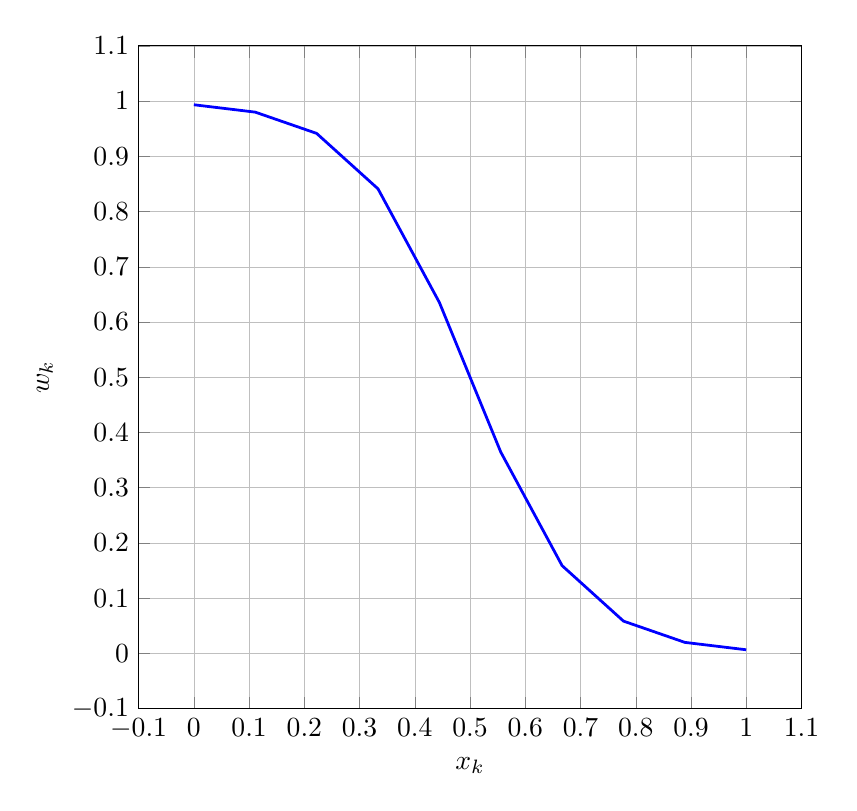
\begin{tikzpicture}[
    declare function={sig(\x) = 1 / (1 + exp(10*(\x - 0.5)));}
   ]
   \begin{axis}[
     unit vector ratio =1 1,
     domain=0:1,
     samples=10,
     yticklabel style={
       /pgf/number format/fixed,
       /pgf/number format/precision=5
      },
     width=10cm,
     height=10cm,
     xtick distance=0.1,
     ytick distance=0.1,
     xlabel={$x_k$},
     ylabel={$w_k$},
     grid=both,
     grid style={
       line width=.1pt,
       draw=gray!10},
     major grid style={
       line width=.2pt,
       draw=gray!50
      },
    ]
    \addplot [color=blue, mark=none,line width=1pt,mark size=1pt] {sig(x)};
   \end{axis}
  \end{tikzpicture}
\end{center}
 \caption{Moving Mirrored Sigmoid Weighted Window of $N=10$ and $\alpha=10$}\label{fig:sigwin}
\end{figure}

\vspace{0.5cm}

To track changes in the input vector $\textbf{u}_k$, we create a fixed $N$ length queue $\textbf{q}_k$ of $\Delta \textbf{u}_k$ elements, to which we enqueue $\Delta \textbf{u}_k =  \textbf{u}_k - \textbf{u}_{k-1}$ before every iteration and dequeue the first element.

In case of $\Delta \textbf{u}_k=0$ the process noise covariance matrix $\textbf{Q}_k$ shoudn't change, so we model it as:
\begin{align*}
    \textbf{Q}_k = \boldsymbol{\Upsilon}_k \textbf{R}_k (1+ \Delta \textbf{Q}_k) \\
\end{align*}
Where:
\begin{align*}
\Delta \textbf{Q}_k &=
\begin{bmatrix}
    \dfrac{M_1}{max(\textbf{q}_k^{\vartheta_k})} \sum_{i=1}^{N} q_{N+1-i}^{\vartheta_k} w_i & 0 \\
    0 & \dfrac{M_2}{max(\textbf{q}_k^{\eta_k})} \sum_{i=1}^{N} q_{N+1-i}^{\eta_k} w_i \\
\end{bmatrix}
\end{align*}

and $M_1, M_2 \in \Re$ are constants, $\textbf{q}_k^{\vartheta_k}, \textbf{q}_k^{\eta_k}$ are the queues corresponding to the input vector $\Delta \textbf{u}_k$.

\end{document}
